\section{Developing}\label{sec:developing}

The application, which has been created, is satisfying the requirements described in problem definition. On picture \ref {fig:classDiagram} the chart of classes of the created program is represented.

\begin{figure}[tbh]
\centering
\caption{The diagram of classes of the developed application }
\label{fig:classDiagram}
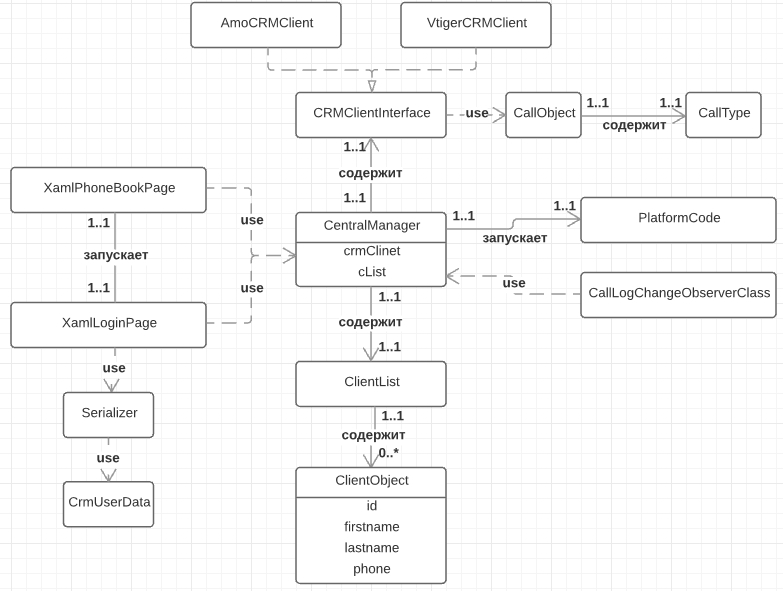
\includegraphics[width=\linewidth]{classDiagram}
\end{figure}

Classes of the application can be divided into four main groups.

The first group of classes is displayed in the left part of picture \ref {fig:classDiagram}. These are the classes which are responsible for the graphic interface and interaction with it. The second group is located on the top of the picture and unites the classes interacting with CRM systems. The third group of classes is responsible for a platform-dependent part of the application and is on the right part of picture \ref {fig:classDiagram}. In the central part of the picture classes of the main logic are represented. Their main task is to realize logic of operation of application and to provide interaction of other three parts. 
